\documentclass[a4paper,class=article,border=10pt,tikz]{standalone}

%mypackages
\usepackage{pythontex}
\usepackage{pgfplots}
\usepackage{amsmath}
\usepackage{titlesec}
\usepackage{tikz}
\usetikzlibrary{shapes.geometric}
\usetikzlibrary{positioning}
\usetikzlibrary{snakes,calc,positioning,patterns,angles,quotes,decorations.pathmorphing,decorations.markings}
% \titleformat{<command>}[<shape>]{<format>}{<label>}{<sep>}{<before-code>}[<after-code>]
%\titleformat{\section}{\normalfont\Large\bfseries}{\thesection.}{10pt}{}
% \titlespacing{<command>}{<left>}{<before-sep>}{<after-sep>}
%\titlespacing{\section}{0pt}{14pt}{7pt}

%\titleformat{\subsection}{\normalfont\itshape}{\thesubsection.}{10pt}{}
%\titlespacing{\subsection}{0pt}{12pt}{6pt}
% set font encoding for PDFLaTeX, XeLaTeX, or LuaTeX
\usepackage{ifxetex,ifluatex}
\if\ifxetex T\else\ifluatex T\else F\fi\fi T%
  \usepackage{fontspec}
\else
  \usepackage[T1]{fontenc}
  \usepackage[utf8]{inputenc}
  \usepackage{lmodern}
\fi

\usepackage{hyperref}


\title{Title of Document}
\author{Name of Author}

% Enable SageTeX to run SageMath code right inside this LaTeX file.
% http://doc.sagemath.org/html/en/tutorial/sagetex.html
% \usepackage{sagetex}

% Enable PythonTeX to run Python – https://ctan.org/pkg/pythontex
% \usepackage{pythontex}

\begin{document}

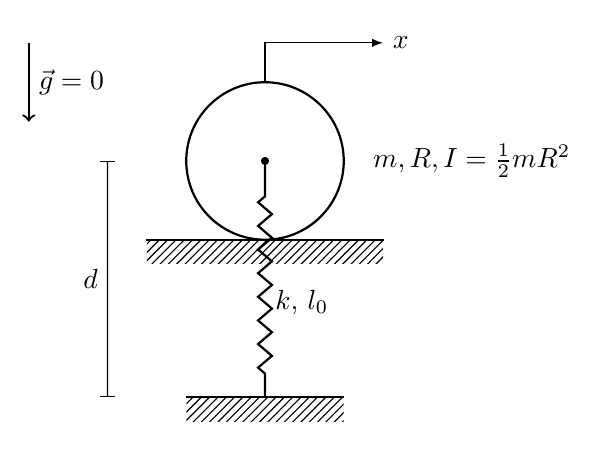
\begin{tikzpicture}[scale=1.0, transform shape]
 \coordinate (origo) at (0,0);

\tikzstyle{spring}=[thick,decorate,decoration={zigzag,pre length=0.3cm,post length=0.3cm,segment length=0.3cm}]

   %draw axes
    \fill[black] (origo) circle (0.05);
    %\draw[thick,gray,->] (origo) -- ++(2,0) node[black,right] {$x$};
    %\draw[thick,gray,->] (origo) -- ++(0,5) node (mary) [black,below] {$y$};
    \draw[thick,<-] (-3,0.5) -- (-3,1.5) node[midway, right] {$\vec{g}=0$};

   %draw roof
    %\fill[pattern = north east lines] ($ (origo) + (-1,0) $) rectangle ($ (origo) + (1,-0.3) $);
    %\draw[thick] ($ (origo) + (-1,-3) $) -- ($ (origo) + (1,-3) $);


    \tikzstyle{ground}=[fill,pattern=north east lines,draw=none,minimum width=0.75cm,minimum height=0.3cm]

    \node (M) [draw,outer sep=0pt,circle,thick,minimum width=2cm, minimum height=2cm,label={[label distance=0.25cm]0:$m, R, I=\frac{1}{2} m R^2$}] {};
    %\node (m1_label) at ($(origo)+(310:3.9cm)$) {$m_{1}$};


    \node (spring_ground) at ($ (M.center) + (0,-3cm) $) {};


    \draw [|-|] (M.center) ++ (-2,0) -- ($(spring_ground.center) + (-2cm,0cm)$) node[midway,left] {$d$};
    \draw [spring] (spring_ground.center) -- (M.center) node [pos=0.4,right] {$k$, $l_{0}$};

    

    
    \fill [black] (M.center) circle (0.05);


    \node (ground) [ground,anchor=north,xshift=-0cm,yshift=-0.cm,minimum width=3cm] at ($(M.south)!0.5!(M.south)$) {};

    \draw [thick] (ground.north west) -- (ground.north east);

    
    
             \node (ground1) [ground,anchor=north,xshift=0cm,yshift=-0cm,minimum width=2cm] at (spring_ground.center) {};

\draw [thick] (ground1.north west) -- (ground1.north east);




\draw [-latex,thin] (M.north) --++ (0cm,0.5cm) -- +(1.5cm,0cm) node[right] {$x$};



\end{tikzpicture}

\end{document}